\section{Cenário Atual}\label{aeb}

A Agência Espacial Brasileira - AEB, autarquia federal vinculada ao Ministério da Ciência e Tecnologia e Inovação - MCTI, criada em 1994, tem a finalidade de promover o desenvolvimento das atividades espaciais de interesse nacional. Compete a ela também dentre vários outras atividades, a formulação e coordenação da política espacial brasileira, de acordo com \cite{Lei:8.854} e \cite{Decreto:4.718}.

Segundo \cite{Decreto:4.718}, a AEB é um dos órgãos que compõem o Sistema Nacional de Desenvolvimento das Atividades Espaciais - SINDAE, que é o conjunto dos órgãos responsáveis pela organização e execução das atividades do Programa Espacial Brasileiro.

As iniciativas e atividades planejadas e em execução pela autarquia, estão organizadas pelo Programa Nacional de Atividades Espaciais - PNAE.

A estrutura organizacional da AEB disponível na Figura~\ref{fig:OrgAeb}.

\begin{figure}[ht]
\centering
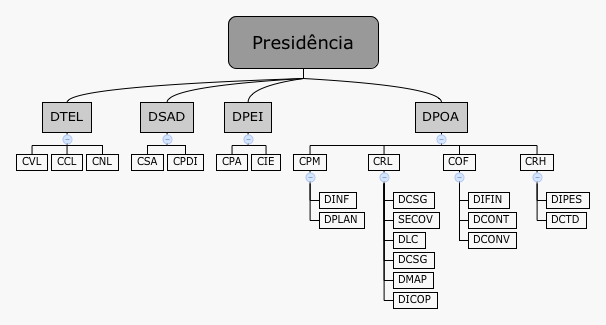
\includegraphics[width=.7\textwidth]{OrgAeb.png}
\caption{Organograma AEB}
\label{fig:OrgAeb}
\end{figure}

A agencia está subdividida em: presidência, diretorias, coordenações e divisões. As diretorias são responsáveis por executar as tarefas do órgão, e segmenta suas atividades na coordenações e divisões. Compete as diretorias de acordo com o \cite{Decreto:4.718}:

\textbf{DTEL} - Diretoria de Transporte Espacial e Licenciamento, compete a diretoria implementar, coordenar e supervisionar projetos e atividades relativos a foguetes, veículos lançadores e centros de lançamento. Como também promover iniciativas de comercialização de bens e serviços espaciais, coordenar a concessão de licenças e autorizações relativas as atividades espaciais. 

\textbf{DSAD} - Diretoria de Satélites, Aplicações e Desenvolvimento, a diretoria é responsável por implementar coordenar e supervisionar os projetos e atividades relativos a satélites espaciais, como também promover a transferência de tecnologia para setor produtivo e promover a integração de instituições de ensino e sua capacitação para atuar em atividades espaciais.
 
\textbf{DPEI} - Diretoria de Política Espacial e Investimentos Estratégicos, compete a diretoria elaboração e atualização do PNAE, identificação de oportunidades e estratégias de investimento no setor espacial e realizar estudos e análises pertinentes à área espacial.

\textbf{DPOA} - Diretoria de Planejamento Orçamento e Administração, a diretoria é responsável por coordenar e controlar a execução das atividade relacionadas aos Sistemas de Pessoal Civil da Administração Federal - SIPEC, de Organização e Modernização Administrativa - SOMAD, de Administração dos Recursos de Informação e Informática - SISP, de Serviços Gerais - SISG, de Planejamento e de Orçamento Federal, de Contabilidade Federal e de Administração Financeira Federal.

Como podemos observar a diretoria responsável pela área de TI é a, DPOA diretoria responsável pela área administrativa do órgão.

\subsection{Tecnologia da Informação - TI da AEB}\label{sec:TIAEB}

A Divisão de Informática - DINF, é subordinada a Coordenação de Planejamento e Modernização - CPM que pertence a DPOA. A divisão é a área responsável por fornecer serviços de TI, e pela gerência dos projetos e atividades relacionadas a TI, desde suporte ao usuário a aquisição de materiais de informática.

A DINF está organizada como mostra a Figura~\ref{fig:orgDinf}.

\begin{figure}[ht]
\centering
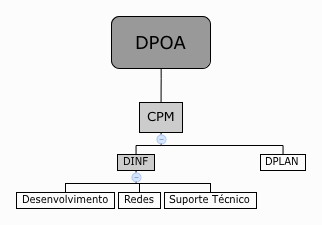
\includegraphics[width=.7\textwidth]{DPOA_dinfAtual.png}
\caption{Organograma DINF}
\label{fig:orgDinf}
\end{figure}

Compete a DINF:

\begin{itemize}
\item Manter Plano Diretor de TI - PDTI;
\item Implementação de metodologias e ferramentas indicadas pelo SISP;
\item Gerência de Informação;
\item Suporte a usuário;
\item Desenvolvimento e manutenção de sistemas administrativos;
\item Desenvolvimento e manutenção de Sitio e Intrnaet da AEB;
\item Análise de viabilidade de implementação de tecnologia;
\item Gerência de redes;
\item Desenvolvimento e manutenção de projetos de redes;
\item Responsável pela implementação de política de segurança digital e 
\item Aquisição de recursos de informática.
\end{itemize}

\subsubsection{iGovTI}

Segundo a definição de IGovTI na Sesão \ref{subsec:iGovTI} o índice avalia a efetividade das ações para medir a Governança de TI nos orãos federais. 

A AEB participa dessa avaliação no qual os resultado vem avançando no indice.  Segundo o \cite{acordaoTCU} os últimos resultados foram:

iGovTI 2012 com 349 participantes foi:

\begin{itemize}
\item 8º lugar, dentre 23 autarquias do governo federal
\item 73º lugar, dentre 214 órgãos do governo federal vinculados ao SISP/MPOG
\item 149º lugar, dentre 349 órgãos do governo federal
\end{itemize}

iGovTI 2014 com 372 participantes é:

\begin{itemize}
\item 7º lugar, dentre 27 autarquias do governo federal
\item 54º lugar, dentre 229 órgãos do governo federal vinculados ao SISP/MPOG
\item 105º lugar, dentre 372 órgãos do governo federal
\end{itemize}

Este índice ajuda a instituição mensurar a importância que a TI exerce no órgão quanto a sua governança e gestão.

\subsection{Cenário Encontrados}

Como já dito na Seção \ref{first:figs}, a TI precisa ser alinhada as estratégias das instituições para que haja alcance satisfatório nos resultados.

A informática na AEB é considerada área meio e é responsável por disponibilizar os serviços da TI aos usuários e os manter em funcionamento. Essa situação evidencia-se ao observar o organograma da DINF na Figura~\ref{fig:orgDinf}, onde as áreas que a compõem são: suporte a aplicação, a equipamentos e serviços que já são fornecidos. Não existe área responsável por identificar as necessidades do negócio, nem quanto a segurança dos dados. Nem existe área ou processo responsável em aplicar a gerência de resposta a riscos.

Alguns problemas existentes:

\begin{itemize}
\item Processos Indefinidos;
\item Recursos humanos insuficientes para atender as demandas;
\item Aplicações inconsistentes com as necessidades do órgão;
\item Falta de estabilidade de serviços fornecidos pela rede.
\end{itemize}

Esses serviços deixam a desejar não pela falta de mão de obra competente, mas pela falta de área responsável dedicada a cada uma das diversas atividades que a TI exerce. 

A dependência do negócio a TI é caracterizado por quanto maior a quantidade de operações chaves dependem da TI, maior é seu papel na organização. Como mostra a Figura~\ref{fig:impactoti} :

\begin{figure}[ht]
\centering
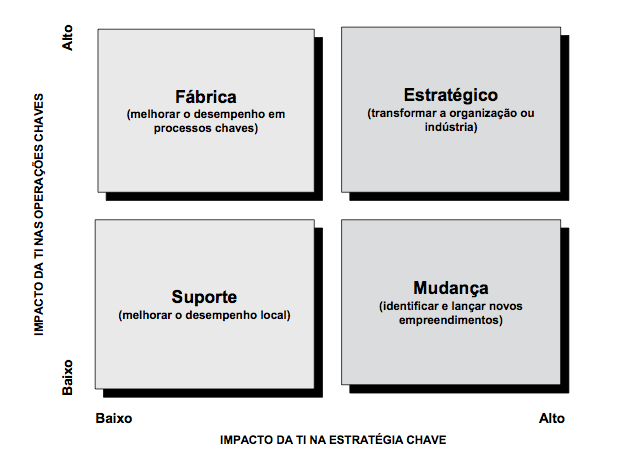
\includegraphics[width=.7\textwidth]{impactoTI.png}
\caption{Impacto estratégico da tecnologia da informação.}
\label{fig:impactoti}
\end{figure}

\begin{itemize}
\item Quando a TI tem alto impacto nas operações chaves e alto impacto nas estratégias chave, ela é estratégica ao negócio.
\item Quando a TI tem alto impacto nas operações chaves e baixo impacto nas estratégias chave, a TI depende do negócio mas o seu futuro não.
\item Quando a TI tem baixo impacto nas operações e alto impacto nas estratégias chave, está apoiando o direcionamento do futuro da organização.
\item Quando a TI tem baixo impacto nas operações chave e baixo impacto nas estratégias chave, a TI está executando tarefas de suporte.
\end{itemize}

Segundo a Figura~\ref{fig:impactoti} disponível em \cite{ImplantandoGTI:2012}, a TI encontrada na AEB é uma TI de suporte, pois tem um baixo valor em operações chave e baixo valor nas estratégias do negócio. É focada em atender demandas dos usuários e em manter os sistemas e seus serviços em funcionamento.
